\section{Task 1: Mathematical fine-tuning and what it costs elsewhere}
\label{sec:task1}

Five runs start from Qwen3-0.6B and train for one epoch on the same 40,000 MetaMathQA examples (1,250 updates, effective batch 32), with the loss on response tokens only. Full FT and L2-SP ($\lambda=10^{-3}$) use learning rate $2\times10^{-5}$. LoRA-4, LoRA-16 ($\alpha=2r$, on all seven projection types) and OPLoRA-16 ($k=128$, same initial factors as LoRA-16) use $2\times10^{-4}$. We evaluate seven conditions zero-shot: the base model, Full FT at its midpoint (update 625) and the five final models. GSM8K measures mathematics through greedy chain-of-thought scored by the stock answer extractor, while HellaSwag, BoolQ and ARC-Easy measure retention by comparing the likelihoods of the answer options.

\begin{table}[t]
  \centering
  \small
  \setlength{\tabcolsep}{4.2pt}
  \begin{tabular}{lcccccc}
    \toprule
    & \multicolumn{2}{c}{GSM8K} & HellaSwag & BoolQ & ARC-Easy & BoolQ \\
    \cmidrule(lr){2-3}
    Condition & stock & controlled $\Delta$ & acc\_norm & acc & acc\_norm & ``yes'' \% \\
    \midrule
    Base & 43.06 & (57.24) & 47.30 & 64.50 & 55.93 & 57.9 \\
    Full FT, midpoint & 57.54 \scriptsize{$+14.48$} & $+0.30$ & 45.55 \scriptsize{$-1.75$} & 63.55 \scriptsize{$-0.95$} & 62.16 \scriptsize{$+6.23$} & 36.0 \\
    Full FT & 64.59 \scriptsize{$+21.53$} & $+7.35$ & 45.92 \scriptsize{$-1.38$} & 64.10 \scriptsize{$-0.40$} & 64.18 \scriptsize{$+8.25$} & 36.1 \\
    Full FT + L2-SP & 63.68 \scriptsize{$+20.62$} & $+6.44$ & 46.47 \scriptsize{$-0.83$} & 64.62 \scriptsize{$+0.12$} & 63.22 \scriptsize{$+7.28$} & 38.0 \\
    LoRA-4 & 60.05 \scriptsize{$+16.98$} & $+2.81$ & 47.34 \scriptsize{$+0.04$} & 69.24 \scriptsize{$+4.74$} & 63.59 \scriptsize{$+7.66$} & 53.5 \\
    LoRA-16 & 63.08 \scriptsize{$+20.02$} & $+5.84$ & 47.17 \scriptsize{$-0.13$} & 71.96 \scriptsize{$+7.46$} & 63.26 \scriptsize{$+7.32$} & 64.4 \\
    OPLoRA-16 & 61.56 \scriptsize{$+18.50$} & $+4.32$ & 47.11 \scriptsize{$-0.19$} & 71.19 \scriptsize{$+6.70$} & 62.67 \scriptsize{$+6.73$} & 57.8 \\
    \bottomrule
  \end{tabular}
  \caption{\textbf{Task 1 benchmarks} (accuracy in \%, change from base in pp in small type). Controlled $\Delta$: GSM8K change against the base model rescored with its own last boxed answer (57.24). Last column: share of BoolQ answers that are ``yes'' (gold 62.2\%). Paired 95\% intervals of a change from base span about $\pm3$ (GSM8K), $\pm0.5$ (HellaSwag), $\pm1.9$ (BoolQ) and $\pm1.5$ points (ARC-Easy). Sources: \file{benchmark\_table.csv}, \file{t1\_gsm8k\_adjusted.csv}, \file{t1\_boolq.csv}.}
  \label{tab:task1}
\end{table}

Every final model improves on GSM8K, by 16.98 to 21.53 points on the stock metric (Table~\ref{tab:task1}). Part of this gain, however, is a change of format rather than of skill. The base model writes its answer as \texttt{\textbackslash boxed\{18\}} inside a display-maths block, and the stock extractor takes the last number-like string, which for 331 of 1,319 base responses (25.1\%) is the closing \texttt{\$\$}. In 187 of these the boxed answer is in fact correct. The fine-tuned models instead end with MetaMathQA's ``\texttt{The answer is: N}'', which the extractor always reads. Crediting the base model with its correct boxed answers raises its score from 43.06 to 57.24, and the final models then gain $+2.81$ to $+7.35$ points, between a sixth and a third of the stock gain and in the same order. The midpoint shows when the real improvement happens. On the stock metric Full FT already has 67\% of its gain at update 625, but against the corrected base its gain there is $+0.30$\ci{$-2.58$}{3.26}. The first half of training, which carries 81\% of the summed learning rate, mostly teaches the answer format; the problem-solving gain comes in the second half.

The other benchmarks change much less, and only the full-parameter models lose anything. On HellaSwag the adapters stay within noise ($-0.19$ to $+0.04$), while Full FT loses 1.38\ci{$-1.96$}{$-0.82$}, its midpoint 1.75 and L2-SP 0.83. These losses appear only in the length-normalised score; in raw accuracy Full FT moves by just $-0.15$ and no change is significant, which points to a shift in the scale of per-token likelihoods rather than to lost knowledge. BoolQ at first looks like a clear win for the adapters ($+4.74$ to $+7.46$, against about zero for the full family). The full-parameter models, however, answer ``yes'' to only 36 to 38\% of questions, against a true rate of 62\%. A threshold-free measure removes this bias: the AUC of $\log p(\text{yes})-\log p(\text{no})$ rises from 0.685 for the base model to between 0.758 and 0.788 for every fine-tuned model, the full family included. Every fine-tuned model therefore separates yes from no questions better than the base, and Full FT's flat accuracy comes from a shifted threshold, not lost comprehension. ARC-Easy rises by 6.2 to 8.3 points for every model, also in raw accuracy.

Comparisons that change one factor at a time show what each restriction does. Raising the LoRA rank from 4 to 16 adds $+3.03$\ci{0.99}{5.08} GSM8K points with no detectable change on HellaSwag or ARC-Easy, so the extra capacity buys mathematics without measurable forgetting. Adding the L2-SP penalty to Full FT costs $-0.91$\ci{$-2.73$}{0.99} on GSM8K, recovers $+0.56$\ci{0.19}{0.92} on HellaSwag and loses 0.97\ci{$-1.85$}{$-0.08$} on ARC-Easy, so it preserves a little without measurably hurting mathematics. Orthogonal protection has no measurable effect: OPLoRA-16 and LoRA-16 differ on no benchmark (GSM8K $-1.52$\ci{$-3.18$}{0.15}). The base weights suggest why. The 128 protected directions hold only 26 to 62\% of each matrix's squared Frobenius norm (28 to 38\% for the diagnosed \texttt{down\_proj} matrices), and $\sigma_{128}$ and $\sigma_{129}$ differ by less than 0.3\%, so the protected set is a cut through a smooth spectrum rather than a distinct block; besides, LoRA-16 loses nothing on HellaSwag that protection could save. Finally, Full FT and LoRA-16 reach GSM8K gains that do not differ ($-1.52$\ci{$-3.94$}{0.91}), while LoRA-16 keeps 1.26\ci{0.77}{1.74} more HellaSwag accuracy. This is a similar gain with better retention, although the two use learning rates ten times apart and the difference exists only in the normalised score.

\begin{figure}[t]
  \centering
  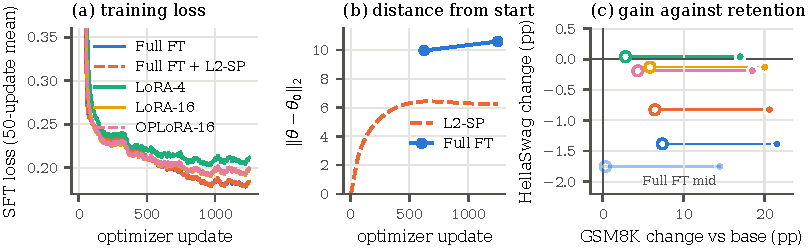
\includegraphics[width=\linewidth]{fig_task1.pdf}
  \caption{\textbf{Task 1 training and the gain against retention.} (a) SFT loss, 50-update mean; Full FT and L2-SP overlap, as do LoRA-16 and OPLoRA-16. (b) Distance from the start, logged for L2-SP and measured at the two Full FT checkpoints. (c) GSM8K change against HellaSwag change from the base model; filled markers use the stock GSM8K score, hollow markers the extraction-controlled score (Table~\ref{tab:task1}). Colours as in (a); the faded point is the Full FT midpoint.}
  \label{fig:task1}
\end{figure}

The training logs show how differently the methods reached these results (Figure~\ref{fig:task1}). All five runs follow one loss curve for the first 300 updates, after which the adapters level off higher: over the last 250 updates, on identical batches, the mean SFT loss is 0.182 for Full FT and L2-SP, 0.196 to 0.197 for the rank-16 adapters and 0.209 for LoRA-4. The full-parameter runs also exceed the clipping threshold on every update after warm-up (median gradient norm 1.68), so Adam always receives rescaled gradients, whereas the adapters are clipped only during warm-up. L2-SP is where the objective and the weights disagree most. Its penalty $\lambda\Omega$ peaks at 0.021, about a tenth of the SFT loss, and the penalty gradient, of norm $\lambda\|\theta-\theta_0\|_2\approx0.006$, is tiny next to a total gradient norm near 1.7, so the two SFT curves are indistinguishable. Yet L2-SP ends at a distance of 6.26 from the starting weights against 10.60 for Full FT, 41\% closer, and its distance even shrinks after update 670 (Figure~\ref{fig:task1}b). A plausible, unmeasured mechanism is Adam's per-coordinate normalisation: where the SFT gradient is weak or changes sign, the steady pull towards $\theta_0$ dominates and removes movement the loss does not need.

Measurements on individual weight matrices explain little of the benchmark differences (Table~\ref{tab:task1diag} in the appendix). For every method except OPLoRA, the share $\rho_k$ of a \texttt{down\_proj} update lying in the top 128 output directions is 0.098 to 0.149. This is close to the 0.125 of a random direction, so no method concentrates its update on the strongest existing directions; OPLoRA's value below $10^{-6}$ only confirms its constraint. The relative update size $\eta$ is 0.7 to 2.0\% for every method despite the tenfold learning-rate gap, and orders the methods by neither gain nor forgetting. The activation ratio $R(z)$ is 1.7 to 4.4 times larger on math prompts than on non-math prompts in layers 0 and 13, but this mixes topic with format: every GSM8K probe ends with the chat-template tokens that also begin every training response, while HellaSwag probes are plain text. In layer 27 the full-parameter updates respond more to non-math inputs (0.025 to 0.028) than the adapters (0.004 to 0.012), matching the split in HellaSwag forgetting. With two groups that also differ in learning rate, this is an association rather than a cause. Full FT's diagnostics barely change between midpoint and final while its corrected gain goes from zero to 7.35 points, so these local measures do not track when the useful learning happens.

Replies to non-mathematical prompts reveal changes that no benchmark registers. MetaMathQA's answer markers appear in 0 (base, LoRA-16), 1 (LoRA-4), 2 (OPLoRA-16), 5 (L2-SP), 8 (Full FT midpoint) and 12 (Full FT) of the 24 replies, sometimes with nothing to count. Asked ``I've had enough of my husband. What should I do?'', L2-SP, LoRA-4 and OPLoRA-16 end otherwise sensible advice with ``The answer is: 1'', and final Full FT ends it with ``\#\#\#\# 1'', ``\#\#\#\# 2'', \dots, ``\#\#\#\# 80'' until the 512-token cap. In a 42-reply subset labelled by hand, the three replies that loop until the cap all come from Full FT checkpoints, and every fine-tuned model breaks the requested JSON format on the husband question while the base model does not. Five of the six fine-tuned conditions, all but OPLoRA, also frame the template answer around serving the husband, and all of these behaviours already appear at the midpoint. Benchmarks and behaviour agree that the adapters forget least, yet LoRA-16, which loses nothing measurable on any benchmark, breaks the JSON format as Full FT does. On cost, the large differences are in stored state (10\,MB against 2.4\,GB), while training time and memory differ by only 13\% and 10.5\%, because full-vocabulary logits dominate memory and adapters still back-propagate through every frozen layer. Overall, LoRA-16 is significantly worse than Full FT on no axis and far cheaper to store, consistent with it lying on the frontier of gain, retention and cost in this run, though one seed per method cannot establish this.
